\documentclass[color=usenames,dvipsnames]{beamer}\usepackage[]{graphicx}\usepackage[]{color}
% maxwidth is the original width if it is less than linewidth
% otherwise use linewidth (to make sure the graphics do not exceed the margin)
\makeatletter
\def\maxwidth{ %
  \ifdim\Gin@nat@width>\linewidth
    \linewidth
  \else
    \Gin@nat@width
  \fi
}
\makeatother

\definecolor{fgcolor}{rgb}{0, 0, 0}
\newcommand{\hlnum}[1]{\textcolor[rgb]{0.69,0.494,0}{#1}}%
\newcommand{\hlstr}[1]{\textcolor[rgb]{0.749,0.012,0.012}{#1}}%
\newcommand{\hlcom}[1]{\textcolor[rgb]{0.514,0.506,0.514}{\textit{#1}}}%
\newcommand{\hlopt}[1]{\textcolor[rgb]{0,0,0}{#1}}%
\newcommand{\hlstd}[1]{\textcolor[rgb]{0,0,0}{#1}}%
\newcommand{\hlkwa}[1]{\textcolor[rgb]{0,0,0}{\textbf{#1}}}%
\newcommand{\hlkwb}[1]{\textcolor[rgb]{0,0.341,0.682}{#1}}%
\newcommand{\hlkwc}[1]{\textcolor[rgb]{0,0,0}{\textbf{#1}}}%
\newcommand{\hlkwd}[1]{\textcolor[rgb]{0.004,0.004,0.506}{#1}}%
\let\hlipl\hlkwb

\usepackage{framed}
\makeatletter
\newenvironment{kframe}{%
 \def\at@end@of@kframe{}%
 \ifinner\ifhmode%
  \def\at@end@of@kframe{\end{minipage}}%
  \begin{minipage}{\columnwidth}%
 \fi\fi%
 \def\FrameCommand##1{\hskip\@totalleftmargin \hskip-\fboxsep
 \colorbox{shadecolor}{##1}\hskip-\fboxsep
     % There is no \\@totalrightmargin, so:
     \hskip-\linewidth \hskip-\@totalleftmargin \hskip\columnwidth}%
 \MakeFramed {\advance\hsize-\width
   \@totalleftmargin\z@ \linewidth\hsize
   \@setminipage}}%
 {\par\unskip\endMakeFramed%
 \at@end@of@kframe}
\makeatother

\definecolor{shadecolor}{rgb}{.97, .97, .97}
\definecolor{messagecolor}{rgb}{0, 0, 0}
\definecolor{warningcolor}{rgb}{1, 0, 1}
\definecolor{errorcolor}{rgb}{1, 0, 0}
\newenvironment{knitrout}{}{} % an empty environment to be redefined in TeX

\usepackage{alltt}
%\documentclass[color=usenames,dvipsnames,handout]{beamer}

\usepackage[roman]{../lectures}
%\usepackage[sans]{../lectures}


\hypersetup{pdfpagemode=UseNone,pdfstartview={FitV}}



\title{Lecture 3 -- Basic statistical models}
\author{Richard Chandler}




% Load function to compile and open PDF


% Compile and open PDF







%<<knitr-setup,include=FALSE,purl=FALSE>>=
%##opts_chunk$set(comment=NA)
%@


%% New command for inline code that isn't to be evaluated
\definecolor{inlinecolor}{rgb}{0.878, 0.918, 0.933}
\newcommand{\inr}[1]{\colorbox{inlinecolor}{\texttt{#1}}}
\IfFileExists{upquote.sty}{\usepackage{upquote}}{}
\begin{document}

% This would affect all code boxes. Not a good idea.
% \setlength\fboxsep{0pt}



\begin{frame}[plain]
  \LARGE
%  \maketitle
  \centering
  {\huge Lecture 3 -- Refresher of basic statistical models} \\
  {\color{default} \rule{\textwidth}{0.1pt}}
  \vfill
  \large
  WILD(FISH) 8390 \\
  Estimation of Fish and Wildlife Population Parameters \\
  \vfill
  \large
  Richard Chandler \\
  University of Georgia \\
\end{frame}




\section{Linear models}


\begin{frame}[plain]
  \frametitle{Today's Topics}
  \Large
  \only<1>{\tableofcontents}%[hideallsubsections]}
  \only<2 | handout:0>{\tableofcontents[currentsection]}%,hideallsubsections]}
\end{frame}




\begin{frame}
  \frametitle{Linear models (LMs)}
\end{frame}



\begin{frame}[fragile]
  \frametitle{Is this a linear model?}
\[
y = 20 + 0.5 x
\]

\begin{center}
  \includegraphics[width=0.6\textwidth]{figure/linmod1-1}
\end{center}
\end{frame}




\begin{frame}[fragile]
  \frametitle{Is this a linear model?}
\[
y = 20 + 0.5 x - 0.3 x^2
\]

\begin{center}
  \includegraphics[width=0.6\textwidth]{figure/linmod2-1}
\end{center}
\end{frame}



\begin{frame}
  \frametitle{Linear models}
  All fixed-effects regression and ANOVA models are linear models \\
  \vfill
  You must understand linear models before you can apply more advanced models such as GLMs, GAMS, GLMMs, etc\dots
  \vfill
  \centering
  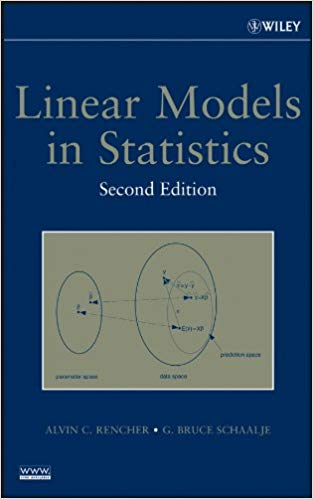
\includegraphics[width=0.25\textwidth]{figure/Rencher_Schaal_book} \hspace{1cm}
  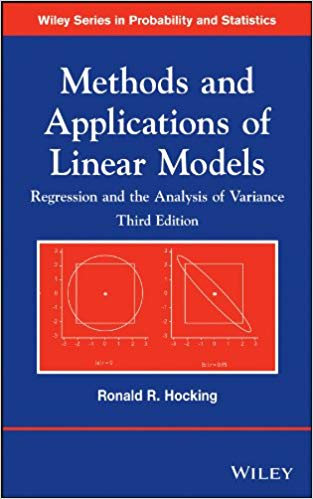
\includegraphics[width=0.25\textwidth]{figure/Hocking_book} \\
\end{frame}



\begin{frame}
  \frametitle{Linear model}
{\bf A linear model is an equation of the form:}

\[
y_i = \beta_0 + \beta_1 x_{i1} + \beta_2 x_{i2} + \ldots + \beta_p x_{ip} + \varepsilon_i
\]

where the $\beta$'s are coefficients, and the $x$ values are predictor
variables (or dummy variables for categorical predictors).
\pause

\vspace{0.5cm}

{\bf This equation is often expressed in matrix notation as:}

\[
{\bf y} = {\bf X} {\bm{\beta}} + {\bm \varepsilon}
\]

where $\bf X$ is a \alert{design matrix} and $\bm{\beta}$ is a
vector of coefficients. \pause More on matrix notation later\dots
\end{frame}


%\end{document}




\begin{frame}
  \frametitle{Interpretting the $\beta$'s}
You must be able to interpret the $\beta$
coefficients {\it for any model that you fit to your data}.
\pause
\vfill
A linear model might have dozens of continuous and categorical
predictors variables, with dozens of associated $\beta$ coefficients.
\pause
\vfill
%% Key points for interpretting $\beta$'s:
%% \begin{itemize}
%%   \item For continuous explano
%% \end{itemize}
Linear models can also include polynomial terms and interactions
\end{frame}


\begin{frame}[fragile]
  \frametitle{Interpretting the $\beta$'s}% for continuous explanatory variables}
  \small 
  The intercept $\beta_0$ is the expected value of $y$, when all $x$'s are 0 \\
  \pause
  \vfill
  If $x$ is a {\bf continuous} explanatory variable: %, $\beta$ is
  \begin{itemize}
    \item $\beta$ can usually be interpretted as a \textit{slope}
      parameter.
    \item In this case, $\beta$ is the
      change in $y$ resulting from a 1 unit change in $x$ (while
      holding the other predictors constant).
    \end{itemize}
\pause
\vfill

\centering
\begin{columns}
  \begin{column}{0.5\textwidth}
\begin{knitrout}\tiny
\definecolor{shadecolor}{rgb}{0.878, 0.918, 0.933}\color{fgcolor}\begin{kframe}
\begin{alltt}
\hlkwd{lm}\hlstd{(y}\hlopt{~}\hlstd{x)}
\end{alltt}
\begin{verbatim}
## 
## Call:
## lm(formula = y ~ x)
## 
## Coefficients:
## (Intercept)            x  
##       9.116        1.032
\end{verbatim}
\end{kframe}
\end{knitrout}
  \end{column}
  \begin{column}{0.4\textwidth}
  \includegraphics[width=\textwidth]{figure/linmod-1} \\
  \end{column}
\end{columns}
\end{frame}




\begin{frame}[fragile]
  \frametitle{\small Interpretting $\beta$'s for categorical explantory variables}
  Things are more complicated for {\bf categorical} explantory
  variables (i.e., factors) because they must be converted to dummy
  variables
  \pause
  \vfill
  There are many ways of creating dummy variables
  \pause
  \vfill
%  For a {\bf categorical} explanatory variable %, $\beta$ is
  In \R, the default method for creating dummy variables from
  unordered factors works like
  this: %unordered factors is called \inr{"contr.treatment"}
  \begin{itemize}
    \item One level of the factor is treated as a \alert{reference level}
    \item The reference level is associated with the intercept
    \item The $\beta$ coefficients for the other levels of the factor
      are differences from the reference level.
  \end{itemize}
  \pause
  \vfill
  The default method corresponds to:
\begin{knitrout}\small
\definecolor{shadecolor}{rgb}{0.878, 0.918, 0.933}\color{fgcolor}\begin{kframe}
\begin{alltt}
\hlkwd{options}\hlstd{(}\hlkwc{contrasts}\hlstd{=}\hlkwd{c}\hlstd{(}\hlstr{"contr.treatment"}\hlstd{,}\hlstr{"contr.poly"}\hlstd{))}
\end{alltt}
\end{kframe}
\end{knitrout}
\end{frame}




\begin{frame}[fragile]
  \frametitle{\small Interpretting $\beta$'s for categorical explantory variables}
  Another common method for creating dummy variables results in
  $\beta$'s that can be interpretted as the $\alpha$'s from the
  additive models that we saw earlier in the class.
  \pause
  \vfill
  With this method:
  \begin{itemize}
    \item The $\beta$ associated with each level of the factor is the
      difference from the intercept
    \item The intercept can be interpetted as the grand mean if the
      continuous variables have been centered
    \item One of the levels of the factor will not be displayed
      because it is redundant when the intercept is estimated
  \end{itemize}
  \pause
  \vfill
  This method corresponds to:
\begin{knitrout}\small
\definecolor{shadecolor}{rgb}{0.878, 0.918, 0.933}\color{fgcolor}\begin{kframe}
\begin{alltt}
\hlkwd{options}\hlstd{(}\hlkwc{contrasts}\hlstd{=}\hlkwd{c}\hlstd{(}\hlstr{"contr.sum"}\hlstd{,}\hlstr{"contr.poly"}\hlstd{))}
\end{alltt}
\end{kframe}
\end{knitrout}
\end{frame}



\subsection{Example}






\section{Generalized linear models}



\begin{frame}[plain]
  \frametitle{Outline}
  \Large
  \tableofcontents[currentsection]
\end{frame}




\begin{frame}
  \frametitle{Generalized linear models (GLMs)}
\end{frame}





\begin{frame}
  \frametitle{Motivation}
  %% {\bf Limitations of linear models}
  %% \begin{itemize}[<+->]
  %%   \item Not appropriate when response variable is discrete
  %%     (e.g. binary)
  %%   \item Sometimes transformations can't make residuals normal
  %%   \item Predictions might not be on the correct scale
  %%   \item Constant variance assumption can be problematic
  %% \end{itemize}
  \large
  \uncover<1->{{\bf Benefits of generalized linear models}}
  \begin{itemize}%[<+->]
    \item<2-> The residuals don't have to be normally distributed
    \item<3-> The response variable can be binary, integer,
      strictly-positive, etc...
    \item<4-> The variance is not assumed to be constant
    \item<5-> Useful for manipulative experiments or observational
      studies, just like linear models.
  \end{itemize}
  \vfill
  \uncover<6->{
  {\bf Examples}
  \begin{itemize}
    \item Presence-absence studies
    \item Studies of survival
    \item Seed germination studies
%    \item Analysis of zero-inflated count data
  \end{itemize}
  }
\end{frame}



\begin{frame}
  \frametitle{Outline}
  {\bf Logistic regression \\}
  \begin{itemize}
    \item The response variable is usually binary and modeled with a
      binomial distribution
      % \begin{itemize}
      %   \item Presence/absence data
      %   \item Yes/no data
      % \end{itemize}
%    \item The response variable is modeled with a binomial distribution
    \item The probability of success is usually a logit-linear
      model
  \end{itemize}
  \pause
  \vfill
  {\bf Poisson regression \\}
  \begin{itemize}
    \item The response variable is a non-negative integer modeled with
      a Poisson distribution
      % \begin{itemize}
      %   \item Count data
      % \end{itemize}
%    \item The response variable is modeled with a Poisson distribution
    \item The expected count is usually modeled with a log-linear
      model
  \end{itemize}
  \vfill
\end{frame}



% \begin{frame}
%   \frametitle{From linear to generalized linear}
% \only<1>{
%   {\bf A linear model is an equation of the form:}
%   \[
%     \mu_i = \beta_0 + \beta_1 x1_i + \beta_2 x2_i + \ldots + \beta_p xp_i
%   \]
%   }
% \only<2>{
%   {\bf A generalized linear model is an equation of the form:}
%   \[
%     g(\eta_i) = \beta_0 + \beta_1 x1_i + \beta_2 x2_i + \ldots + \beta_p xp_i
%   \]
%   }
% \end{frame}


\begin{frame}
  \frametitle{From linear to generalized linear}
  {\bf Linear model}
  \begin{gather*}
    \mu_i = \beta_0 + \beta_1 x_{i1} + \beta_2 x_{i2} + \cdots \\
    y_i \sim \mathrm{Normal}(\mu_i, \sigma^2)
  \end{gather*}
  \pause
  \vfill
  {\bf Generalized Linear model}
  \begin{gather*}
    g(\mu_i) = \beta_0 + \beta_1 x_{i1} + \beta_2 x_{i2} + \cdots \\
    y_i \sim f(\mu_i)
  \end{gather*}
  \pause
  {\bf where} \\
  $g$ is a link function, such as the log or logit link \\
  \pause
  $f$ is a probability distribution such as the binomial or Poisson
%  that determines (usually) the variance %(there is no $\sigma^2$ parameter!)
\end{frame}


\begin{frame}
  \frametitle{Alternative representations}
  {\bf This:}
  \begin{gather*}
    g(\mu_i) = \beta_0 + \beta_1 x_{i1} + \beta_2 x_{i2} + \cdots \\
    y_i \sim f(\mu_i)
  \end{gather*}
  \pause
  {\bf Is the same as this:}
  \begin{gather*}
    \mu_i = g^{-1}(\beta_0 + \beta_1 x_{i1} + \beta_2 x_{i2} + \cdots) \\
    y_i \sim f(\mu_i)
  \end{gather*}
  \pause
  {\bf Is the same as this:}
  \begin{gather*}
    g(\mu_i) = {\bf X}{\bm \beta} \\
    y_i \sim f(\mu_i)
  \end{gather*}
\end{frame}


\begin{frame}
  \frametitle{Link functions}
%  \begin{itemize}[<+->]
%    \item
  An inverse link function ($g^{-1}$) transforms values from the $(-\infty,\infty)$
  scale to the scale of interest, such as $(0,1)$ for probabilities  \\
  \pause
  \vfill
%    \item
  The link function ($g$) does the reverse \\
%    \item
%  \pause
%  \vfill
%  The two link functions that you will see most often are the
%      ``logit'' and ``log'' links.
%  \end{itemize}
\end{frame}


\begin{frame}
  \frametitle{Link functions}
  \begin{tabular}{llcc}
    \hline
    Distribution & link name\footnote{\scriptsize These are the most common link functions, but others are available} & link equation             & inverse link equation       \\
    \hline
%    Normal       & identity  & $\mu$                     & ${\bf X}{\bm \beta}$  \\
%                 &           &                           &                             \\
    Binomial     & logit     & $\log(\frac{p}{1-p})$ & $\frac{\exp({\bf
          X}{\bm \beta})}{1 + \exp({\bf X}{\bm \beta})}$                        \\
                 &           &                           &                             \\
    Poisson      & log       & $\log(\lambda)$               & $\exp({\bf X}{\bm \beta})$  \\
    \hline
  \end{tabular}

\pause
\vfill

\begin{tabular}{llcc}
    \hline
    Distribution & link name & link in {\bf R}  & inv link in {\bf R}       \\
    \hline
    Binomial     & logit     & {\tt qlogis} & {\tt plogis}                        \\
                 &           &                           &                             \\
    Poisson      & log       & {\tt log}    & {\tt exp}  \\
    \hline
  \end{tabular}
\end{frame}






%% \begin{frame}[fragile]
%%   \frametitle{Log link example}
%% <<>>=
%% beta0 <- 5
%% beta1 <- -0.08
%% elevation <- 100
%% eta <- beta0 + beta1*elevation
%% eta
%% @
%% \pause
%% {\bf How do we convert -3 to a positive value? \par}
%% \pause
%% {\bf Use the inverse-log function, i.e. the exponential function:}
%% <<>>=
%% exp(-3)
%% @
%% \end{frame}






\begin{frame}[fragile]
  \frametitle{Logit link example}
  \vspace{-5pt}
  \scriptsize
\begin{knitrout}\tiny
\definecolor{shadecolor}{rgb}{0.878, 0.918, 0.933}\color{fgcolor}\begin{kframe}
\begin{alltt}
\hlstd{beta0} \hlkwb{<-} \hlnum{5}
\hlstd{beta1} \hlkwb{<-} \hlopt{-}\hlnum{0.08}
\hlstd{elevation} \hlkwb{<-} \hlnum{100}
\hlstd{(logit.p} \hlkwb{<-} \hlstd{beta0} \hlopt{+} \hlstd{beta1}\hlopt{*}\hlstd{elevation)}
\end{alltt}
\begin{verbatim}
## [1] -3
\end{verbatim}
\end{kframe}
\end{knitrout}
\pause
{How do we convert -3 to a probability? \pause Use the
  inverse-link: \\}
\begin{knitrout}\tiny
\definecolor{shadecolor}{rgb}{0.878, 0.918, 0.933}\color{fgcolor}\begin{kframe}
\begin{alltt}
\hlstd{p} \hlkwb{<-} \hlkwd{exp}\hlstd{(logit.p)}\hlopt{/}\hlstd{(}\hlnum{1}\hlopt{+}\hlkwd{exp}\hlstd{(logit.p))}
\hlstd{p}
\end{alltt}
\begin{verbatim}
## [1] 0.04742587
\end{verbatim}
\end{kframe}
\end{knitrout}
\pause
{Same as:}
\begin{knitrout}\tiny
\definecolor{shadecolor}{rgb}{0.878, 0.918, 0.933}\color{fgcolor}\begin{kframe}
\begin{alltt}
\hlkwd{plogis}\hlstd{(logit.p)}
\end{alltt}
\begin{verbatim}
## [1] 0.04742587
\end{verbatim}
\end{kframe}
\end{knitrout}
\pause
{To go back, use the link function itself:}
\begin{knitrout}\tiny
\definecolor{shadecolor}{rgb}{0.878, 0.918, 0.933}\color{fgcolor}\begin{kframe}
\begin{alltt}
\hlkwd{log}\hlstd{(p}\hlopt{/}\hlstd{(}\hlnum{1}\hlopt{-}\hlstd{p))}
\end{alltt}
\begin{verbatim}
## [1] -3
\end{verbatim}
\begin{alltt}
\hlkwd{qlogis}\hlstd{(p)}
\end{alltt}
\begin{verbatim}
## [1] -3
\end{verbatim}
\end{kframe}
\end{knitrout}
\end{frame}



\begin{frame}[fragile]
  \frametitle{Logit link example}
\begin{knitrout}\scriptsize
\definecolor{shadecolor}{rgb}{0.878, 0.918, 0.933}\color{fgcolor}\begin{kframe}
\begin{alltt}
\hlkwd{plot}\hlstd{(}\hlkwa{function}\hlstd{(}\hlkwc{x}\hlstd{)} \hlnum{5} \hlopt{+ -}\hlnum{0.08}\hlopt{*}\hlstd{x,} \hlkwc{from}\hlstd{=}\hlnum{0}\hlstd{,} \hlkwc{to}\hlstd{=}\hlnum{100}\hlstd{,}
     \hlkwc{xlab}\hlstd{=}\hlstr{"Elevation"}\hlstd{,} \hlkwc{ylab}\hlstd{=}\hlstr{"logit(prob of occurrence)"}\hlstd{)}
\end{alltt}
\end{kframe}
\end{knitrout}
%\begin{center}
\centering
  \includegraphics[width=\textwidth]{figure/nologit-1} \\
%\end{center}
\end{frame}




\begin{frame}[fragile]
  \frametitle{Logit link example}
\begin{knitrout}\scriptsize
\definecolor{shadecolor}{rgb}{0.878, 0.918, 0.933}\color{fgcolor}\begin{kframe}
\begin{alltt}
\hlkwd{plot}\hlstd{(}\hlkwa{function}\hlstd{(}\hlkwc{x}\hlstd{)} \hlkwd{plogis}\hlstd{(}\hlnum{5} \hlopt{+ -}\hlnum{0.08}\hlopt{*}\hlstd{x),} \hlkwc{from}\hlstd{=}\hlnum{0}\hlstd{,} \hlkwc{to}\hlstd{=}\hlnum{100}\hlstd{,}
     \hlkwc{xlab}\hlstd{=}\hlstr{"Elevation"}\hlstd{,} \hlkwc{ylab}\hlstd{=}\hlstr{"Probability of occurrence"}\hlstd{)}
\end{alltt}
\end{kframe}
\end{knitrout}
%\begin{center}
\centering
  \includegraphics[width=\textwidth]{figure/logit2-1} \\
%\end{center}
\end{frame}





\subsection{Logistic regression}


\begin{frame}
  \frametitle{Logistic Regression}
%  \begin{itemize}%[<+->]
%    \item<1->
  Logistic regression is a specific type of GLM in which the
      response variable follows a binomial distribution and the link
      function is the logit \\
  \pause
  \vfill
%    \item<2->
  It would be better to call it ``binomial regression'' since other
      link functions (e.g. the probit) can be used \\
%    \item<3->
  \pause
  \vfill
  Appropriate when the response is binary or a count with an
  upper limit
%    \item<4->
  \pause
  \vfill
  {\bf Examples:}
      \begin{itemize}
        \normalsize
        \item Presence/absence studies
        \item Survival studies
        \item Disease prevalance studies
      \end{itemize}
%  \end{itemize}
\end{frame}



%\begin{frame}[fragile]
%  \frametitle{Logistic Regression}

%\end{frame}



\begin{frame}
  \frametitle{Logistic Regression}
    \begin{gather*}
      \mathrm{logit}(p_i) = \beta_0 + \beta_1 x_{i1} + \beta_2 x_{i2} + \cdots \\
      y_i \sim \mathrm{Binomial}(N, p_i)
  \end{gather*}
  \pause
  {\bf where: \\}
  $N$ is the number of ``trials'' (e.g. coin flips) \\
  $p_i$ is the probability of success for sample unit $i$
\end{frame}



\begin{frame}[fragile]
  \frametitle{Binomial distribution}% - fair coin}
  \vspace{-0.4cm}
  \note{Have students flip coins}
\begin{center}
\begin{knitrout}
\definecolor{shadecolor}{rgb}{0.878, 0.918, 0.933}\color{fgcolor}
\includegraphics[width=0.9\textwidth]{figure/binom1-1} 

\end{knitrout}
\end{center}
\vfill
\end{frame}



\begin{frame}[fragile]
  \frametitle{Binomial distribution}% - warped coin}
  \vspace{-0.4cm}
\begin{center}
\begin{knitrout}
\definecolor{shadecolor}{rgb}{0.878, 0.918, 0.933}\color{fgcolor}
\includegraphics[width=0.9\textwidth]{figure/binom2-1} 

\end{knitrout}
\end{center}
\end{frame}




\begin{frame}
  \frametitle{Binomial Distribution}
  {\bf Properties}
  \begin{itemize}
    \item The expected value of $y$ is $Np$
    \item The variance is $Np(1-p)$
  \end{itemize}
  \pause
  \vfill
  {\bf Bernoulli distribution}
  \begin{itemize}
    \item The Bernoulli distribution is a binomial distribution with a
      single trial ($N=1$)
%    \item Think of it as a single coin flip
    \item Logistic regression is usually done in this context, such
      that the response variable is 0/1 or No/Yes or Bad/Good, etc$\dots$
  \end{itemize}
\end{frame}


% \section{The {\tt glm} function}

\subsubsection{Example}





\subsection{Poisson regression}



\begin{frame}
  \frametitle{Poisson Regression}
  \Large
    \begin{gather*}
      \mathrm{log}(\lambda_i) = \beta_0 + \beta_1 x_{i1} + \beta_2 x_{i2} + \cdots \\
      y_i \sim \mathrm{Poisson}(\lambda_i)
  \end{gather*}
  \pause
  {\bf where: \\}
  $\lambda_i$ is the expected value of $y_i$ \\
\end{frame}



\begin{frame}
  \frametitle{Poisson regression}
  \large
  {\bf Useful for:}
  \begin{itemize}
    \item Count data
    \item Number of events in time intervals
    \item Other types of integer data
  \end{itemize}
  \pause
  \vfill
  {\bf Properties}
  \begin{itemize}
    \item The expected value of $y$ ($\lambda$) is equal to the variance
    \item This is an assumption of the Poisson model
    \item Like all assumptions, it can be relaxed if you have enough data
  \end{itemize}
\end{frame}




\begin{frame}[fragile]
  \frametitle{Poisson distribution}



\begin{center}
  \only<1>{\includegraphics[width=0.75\textwidth]{figure/pois1-1}}
  \only<2 | handout:0>{\includegraphics[width=0.75\textwidth]{figure/pois2-1}}
  \only<3 | handout:0>{\includegraphics[width=0.75\textwidth]{figure/pois3-1}}
\end{center}
\end{frame}









\begin{frame}[fragile]
  \frametitle{Log link example}
  \footnotesize
\begin{knitrout}\footnotesize
\definecolor{shadecolor}{rgb}{0.878, 0.918, 0.933}\color{fgcolor}\begin{kframe}
\begin{alltt}
\hlkwd{plot}\hlstd{(}\hlkwa{function}\hlstd{(}\hlkwc{x}\hlstd{)} \hlnum{5} \hlopt{+ -}\hlnum{0.08}\hlopt{*}\hlstd{x,} \hlkwc{from}\hlstd{=}\hlnum{0}\hlstd{,} \hlkwc{to}\hlstd{=}\hlnum{100}\hlstd{,}
     \hlkwc{xlab}\hlstd{=}\hlstr{"Elevation"}\hlstd{,} \hlkwc{ylab}\hlstd{=}\hlstr{"log(Expected abundance)"}\hlstd{)}
\end{alltt}
\end{kframe}
\end{knitrout}
\begin{center}
  \includegraphics[width=0.8\textwidth]{figure/nolog-1}
\end{center}
\end{frame}




\begin{frame}[fragile]
  \frametitle{Log link example}
  \footnotesize
\begin{knitrout}\footnotesize
\definecolor{shadecolor}{rgb}{0.878, 0.918, 0.933}\color{fgcolor}\begin{kframe}
\begin{alltt}
\hlkwd{plot}\hlstd{(}\hlkwa{function}\hlstd{(}\hlkwc{x}\hlstd{)} \hlkwd{exp}\hlstd{(}\hlnum{5} \hlopt{+ -}\hlnum{0.08}\hlopt{*}\hlstd{x),} \hlkwc{from}\hlstd{=}\hlnum{0}\hlstd{,} \hlkwc{to}\hlstd{=}\hlnum{100}\hlstd{,}
     \hlkwc{xlab}\hlstd{=}\hlstr{"Elevation"}\hlstd{,} \hlkwc{ylab}\hlstd{=}\hlstr{"Expected abundance"}\hlstd{)}
\end{alltt}
\end{kframe}
\end{knitrout}
\begin{center}
  \includegraphics[width=0.8\textwidth]{figure/log-1}
\end{center}
\end{frame}






\begin{frame}
  \frametitle{Assessing model fit}
  {The most common problem in Poisson regression is
    {\alert{overdispersion}}. \\}
  \pause
  \vfill
  {Overdispersion is the situation in which there is more variability
    in the data than predicted by the model. \\}
  \pause
  \vfill
  {Overdispersion cannot be assessed by simply comparing the mean and
    variance of the response variable. \\}
  \pause
  \vfill
  {The presence of many zeros is not necessarily
    indicative of overdispersion. \\}
  \pause
  \vfill
  {Overdispersion can be assessed using a goodness-of-fit test. \\}
\end{frame}



\begin{frame}[fragile]
  \frametitle{Goodness-of-fit}
The fit of a Poisson regression can be assessed using a $\chi^2$
test. \\
\pause
\vfill
The test statistic is the residual deviance:
\[
  D = 2 \left\{\sum y_i \log\left(\frac{y_i}{\hat{\lambda_i}}\right) - (y_i-\hat{\lambda}_i)\right\}
\]
\pause
\vfill
If the null hypothesis is true (ie, the model fits the data), $D$ should
follow $\chi^2$ distribution with $N-K$ degrees-of-freedom.
\pause
\vfill
\begin{knitrout}\footnotesize
\definecolor{shadecolor}{rgb}{0.878, 0.918, 0.933}\color{fgcolor}\begin{kframe}
\begin{alltt}
\hlstd{N} \hlkwb{<-} \hlkwd{nrow}\hlstd{(frogData)}                   \hlcom{# sample size}
\hlstd{K} \hlkwb{<-} \hlkwd{length}\hlstd{(}\hlkwd{coef}\hlstd{(fm2))}                \hlcom{# number of parameters}
\hlstd{df.resid} \hlkwb{<-} \hlstd{N}\hlopt{-}\hlstd{K}                       \hlcom{# degrees-of-freedom}
\hlstd{Dev} \hlkwb{<-} \hlkwd{deviance}\hlstd{(fm2)}                  \hlcom{# residual deviance}
\hlstd{p.value} \hlkwb{<-} \hlnum{1}\hlopt{-}\hlkwd{pchisq}\hlstd{(Dev,} \hlkwc{df}\hlstd{=df.resid)} \hlcom{# p-value}
\hlstd{p.value}                               \hlcom{# fail to reject H0}
\end{alltt}
\end{kframe}
\end{knitrout}
\end{frame}





\begin{frame}
  \frametitle{What if model doesn't fit the data?}
  \Large
  {\bf Alternatives to the Poisson distribution}
  \begin{itemize}
    \item Negative binomial
    \item Zero-inflated Poisson
  \end{itemize}
\end{frame}





\begin{frame}
  \frametitle{Negative binomial distribution}



\begin{center}
  \only<1>{\includegraphics[width=0.75\textwidth]{figure/nb1-1}}
  \only<2 | handout:0>{\includegraphics[width=0.75\textwidth]{figure/nb2-1}}
  \only<3 | handout:0>{\includegraphics[width=0.75\textwidth]{figure/nb3-1}}
\end{center}
\end{frame}




\section{Mixed effects models}



\begin{frame}[plain]
  \frametitle{Outline}
  \Large
  \tableofcontents[currentsection]
\end{frame}




\begin{frame}
  \frametitle{Generalized linear mixed effects models (GLMMs)}
\end{frame}





\begin{frame}
  \frametitle{Fixed vs random effects, revisited}
%  \large
  {\bf In the context of mixed-effects models\dots \par}
  \vspace{0.5cm}
{\bf Fixed effect \par}
A parameter that would not change if you repeated your study

\pause
\vspace{1cm}

{\bf Random effect \par}
A parameter that would change if you repeated your study

\pause
\vfill
{\centering \bf
\alert{Random effects will always be associated with a probability
distribution} \par}
\end{frame}



\begin{frame}
  \frametitle{Previous examples}
  \Large
%  \begin{itemize}
%    \item
  ANOVA with random block effects
  \pause
  \vfill
%    \item[]
%    \item
  Nested ANOVA
  \pause
  \vfill
%    \item[]
%    \item
  Split-plot ANOVA
%    \item[]
%    \item Repeated measures ANOVA
%  \end{itemize}
\end{frame}




\begin{frame}
  \frametitle{A simple example}
  \large
  \[
    y_{ij} = \beta_0 + \beta_1 x_{i1} + \gamma_j + \varepsilon_{ij}
  \]
  where
  \[
    \gamma_j \sim \mbox{Normal}(0, \sigma^2_d)
  \]
  and
  \[
    \varepsilon_{ij} \sim \mbox{Normal}(0, \sigma^2)
  \]
  \pause
  \vfill
  \centering
  This amounts to a linear regression with a random intercept \\
\end{frame}






%% \begin{frame}
%%   \frametitle{Split-plot model}
%%   The expanded additive model:
%%   \[
%%     y_{ijk} = \beta0 + \beta_1 + \beta_{ij} + \gamma_k +
%%     \alpha\gamma_{ik} + \varphi y_{ijk-1} + \varepsilon_{ijk}
%%   \]
%% \end{frame}







\begin{frame}
  \frametitle{Matrix representation}
  \Large
  \[
    {\bf y} = {\bf X}{\bm \beta} + {\bm \gamma} + {\bm \varepsilon}
  \]
  \pause
  \[
    {\bm \gamma} \sim \mbox{Normal}(0, \sigma^2_d)
  \]
  \[
    {\bm \varepsilon} \sim \mbox{Normal}(0, \sigma^2)
  \]
\end{frame}









\section{Summary}


\begin{frame}
  \frametitle{Summary}
  \large
%  \begin{itemize}[<+->]
%    \item
  Linear mixed-effects models are useful anytime you have
  fixed effects and normally-distriubted random effects \\
  \pause
  \vfill
%    \item
  They allow for (serial, spatial, etc\dots) correlation among
  observations within a level of the grouping variable \\
  \pause
  \vfill
%    \item
  These models can be used for repeated measures data as an
  alternative to MANOVA or the split-plot method with adjusted
  $P$-values \\
  \pause
  \vfill
%    \item
  We do not want you to use this approach for the repeated
  measures questions in the exam. \\
  \pause
  \vfill
%    \item
  But we will expect you to know how to fit linear
      mixed-effects models using {\tt lme}, as we have already done
%  \end{itemize}
\end{frame}







\end{document}
